%% Begin the document based on the review and published state
\documentclass[sigconf,]{acmart}

% Make Pandoc happy
  

%% \BibTeX command to typeset BibTeX logo in the docs
\AtBeginDocument{%
  \providecommand\BibTeX{{%
    \normalfont B\kern-0.5em{\scshape i\kern-0.25em b}\kern-0.8em\TeX}}}

\usepackage{booktabs}
\usepackage{caption}   % http://mirror.easyname.at/ctan/macros/latex/contrib/caption/caption-eng.pdf

\usepackage{balance}  % balancing bibstyles as per request in accepted submission
\usepackage{graphicx}
% % We will generate all images so they have a width \maxwidth. This means
% % that they will get their normal width if they fit onto the page, but
% % are scaled down if they would overflow the margins.
\makeatletter
\def\maxwidth{\ifdim\Gin@nat@width>\linewidth\linewidth
\else\Gin@nat@width\fi}
\makeatother
\let\Oldincludegraphics\includegraphics
\renewcommand{\includegraphics}[1]{\Oldincludegraphics[width=\maxwidth]{#1}}

%% These commands are for a PROCEEDINGS abstract or paper.
\copyrightyear{2022}
\acmYear{2022}
\setcopyright{acmcopyright}
\acmConference[Woodstock '22]{Woodstock '22: ACM Symposium on Neural
Gaze Detection}{June 03--05, 2022}{Woodstock, NY}
\acmBooktitle{}
\acmPrice{}
\acmISBN{}
\acmDOI{10.1145/1122445.1122456}

\makeatletter
\@ifpackageloaded{subfig}{}{\usepackage{subfig}}
\@ifpackageloaded{caption}{}{\usepackage{caption}}
\captionsetup[subfloat]{margin=0.5em}
\AtBeginDocument{%
\renewcommand*\figurename{Figure}
\renewcommand*\tablename{Table}
}
\AtBeginDocument{%
\renewcommand*\listfigurename{List of Figures}
\renewcommand*\listtablename{List of Tables}
}
\newcounter{pandoccrossref@subfigures@footnote@counter}
\newenvironment{pandoccrossrefsubfigures}{%
\setcounter{pandoccrossref@subfigures@footnote@counter}{0}
\begin{figure}\centering%
\gdef\global@pandoccrossref@subfigures@footnotes{}%
\DeclareRobustCommand{\footnote}[1]{\footnotemark%
\stepcounter{pandoccrossref@subfigures@footnote@counter}%
\ifx\global@pandoccrossref@subfigures@footnotes\empty%
\gdef\global@pandoccrossref@subfigures@footnotes{{##1}}%
\else%
\g@addto@macro\global@pandoccrossref@subfigures@footnotes{, {##1}}%
\fi}}%
{\end{figure}%
\addtocounter{footnote}{-\value{pandoccrossref@subfigures@footnote@counter}}
\@for\f:=\global@pandoccrossref@subfigures@footnotes\do{\stepcounter{footnote}\footnotetext{\f}}%
\gdef\global@pandoccrossref@subfigures@footnotes{}}
\@ifpackageloaded{float}{}{\usepackage{float}}
\floatstyle{ruled}
\@ifundefined{c@chapter}{\newfloat{codelisting}{h}{lop}}{\newfloat{codelisting}{h}{lop}[chapter]}
\floatname{codelisting}{Listing}
\newcommand*\listoflistings{\listof{codelisting}{List of Listings}}
\makeatother

% 

\begin{document}

% 
  \title{A Paper submitted to a conference}

\author{Jens A. Ewald}
\orcid{0000-0001-6926-9882}
\authornote{All authors contributed equally to this research.}
\email{jens.a.ewald@northumbria.ac.uk}
\affiliation{
    \institution{University of Northumbria}
        \city{Newcastle upon Tyne}
      \country{United Kingdom}
  }
\author{Jayne Wallace}
\email{j.wallace@northumbria.ac.uk}
\affiliation{
    \institution{University of Northumbria}
        \city{Newcastle upon Tyne}
      \country{United Kingdom}
  }
\author{Sahil Thappa}
\authornotemark[1]
\email{}
\affiliation{
    \institution{National Institue for Design}
        \city{Ahmedabad}
      \country{India}
  }

\begin{abstract}
A clear and well-documented \LaTeX~{[}1{]} document is presented as an
article formatted for publication by ACM in a conference proceedings or
journal publication. Based on the ``acmart'\,' document class, this
article presents and explains many of the common variations, as well as
many of the formatting elements an author may use in the preparation of
the documentation of their work.
\end{abstract}

\renewcommand{\shortauthors}{}

\maketitle


\keywords{plaintext, academic publishing, markdown}

% Main body of the document
\hypertarget{introduction}{%
\section{Introduction}\label{introduction}}

I had this initia l idea of being able to write Markdown documents. A
very leighty weight markup for plain text documents would make it easier
and less resource intensive to write. Furthermore, I do take my notes in
this style of writing.

A first research brought me to a blog post {[}2{]} outlining a simple
setup to produce shareable versions of a note as an article in PDF,
HTML, and DOCX.

Ullamco pariatur nostrud commodo ullamco magna ea. Non et magna magna
dolor officia do proident cillum eiusmod reprehenderit irure laborum sit
mollit. Elit ipsum esse non irure proident magna fugiat reprehenderit
laborum quis id pariatur velit cillum. Elit qui esse dolore sint ex
aliquip proident mollit minim dolore esse qui. Deserunt mollit elit nisi
dolore est ad deserunt.\footnote{Foot notes can also be inlined.}

Eiusmod laborum ipsum pariatur veniam eu non quis exercitation minim
commodo incididunt consequat. Adipisicing sunt veniam do magna. Enim
elit adipisicing nulla ad Lorem ea reprehenderit ullamco proident
reprehenderit eu. Id anim est aliqua ut anim ut velit et cupidatat minim
incididunt in. Labore velit in enim minim consequat exercitation Lorem
do sunt exercitation ad do aliquip. Elit velit Lorem veniam mollit est
sint aute excepteur exercitation et. Amet quis cillum fugiat ex.

\hypertarget{preconditions}{%
\section{Preconditions}\label{preconditions}}

Amet excepteur cupidatat incididunt excepteur labore deserunt
exercitation eiusmod sit irure nisi voluptate. Mollit ullamco dolor
dolore quis esse magna adipisicing laboris nostrud fugiat cupidatat
exercitation dolore. Lorem ipsum ad exercitation incididunt nisi sint
pariatur eu aliquip et laboris. Id labore veniam elit consequat
consectetur sit minim nulla. Ut proident proident nulla excepteur ex
ullamco. Culpa ea reprehenderit eu pariatur nisi ex. In laborum culpa ea
anim labore ipsum et sunt.

Qui tempor ipsum voluptate cupidatat incididunt nisi exercitation
occaecat nisi occaecat qui dolore ullamco enim. Dolor veniam cillum duis
aliquip in ut deserunt enim. Reprehenderit cupidatat nostrud irure amet
sint ea adipisicing labore veniam dolore Lorem reprehenderit.{[}3{]}

\hypertarget{how-it-looks-in-practice}{%
\section{How it looks in practice}\label{how-it-looks-in-practice}}

Magna occaecat fugiat aliquip reprehenderit qui exercitation pariatur
cillum tempor. Culpa quis irure laborum mollit nulla culpa sunt do dolor
adipisicing id adipisicing exercitation. Mollit amet nostrud voluptate
tempor cillum enim Lorem quis culpa pariatur officia non occaecat. Non
amet sit adipisicing et non occaecat Lorem est ex aliqua enim pariatur
dolore nisi. Velit Lorem nulla irure anim occaecat consequat enim ut ut
Lorem (as show in fig.~\ref{fig:vscode-view}).

\begin{figure}
\hypertarget{fig:vscode-view}{%
\centering
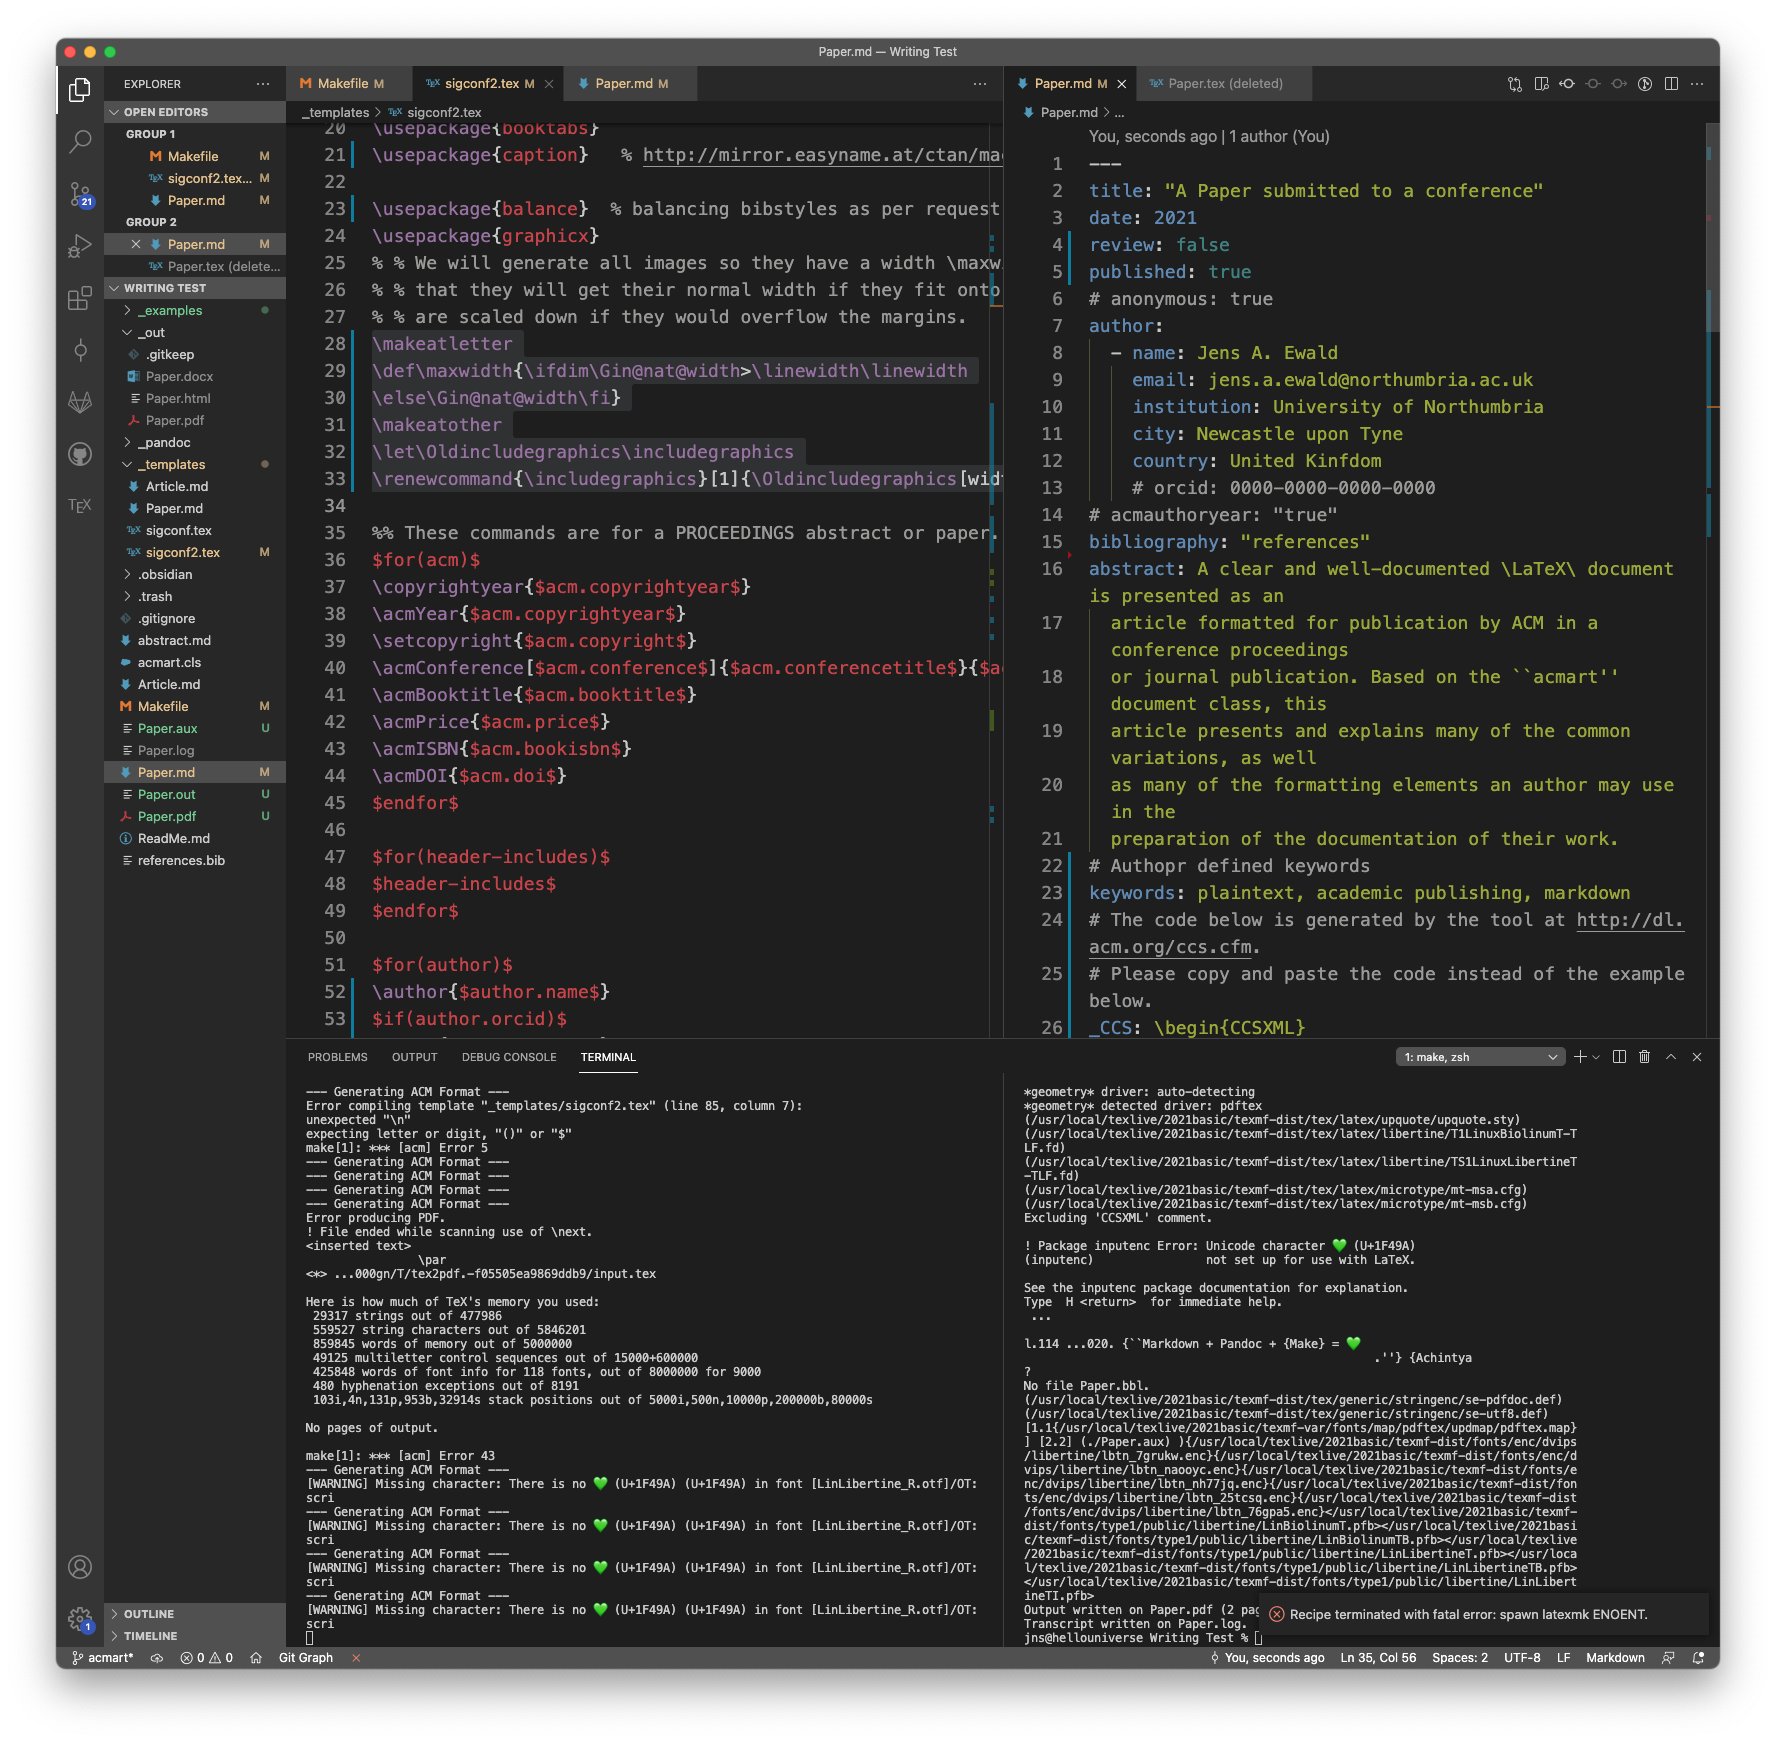
\includegraphics{images/vscode-view.png}
\caption{Editing a template in Visual Studio
Code.}\label{fig:vscode-view}
}
\end{figure}

  \section{References}
  \balance
  \bibliographystyle{ACM-Reference-Format}
  \bibliography{references.bib}

\end{document}
\endinput
